\chapter{Overview of Other \bbbb Channels}
\label{app:other-channels}
The results discussed above have been developed in conjunction with (1) a boosted channel 
for the resonant search and (2) a vector boson fusion (VBF) channel for the non-resonant search. 
Detailed discussions of these two channels are beyond the scope of this thesis, though a 
combined set of resolved and boosted results are presented below. The VBF results are 
not included in this thesis, but much of this thesis work has been useful in the development 
of that result. For completeness, we therefore briefly summarize both analyses here.

\subsection{Resonant: Boosted Channel}
The boosted analysis selection targets resonance masses from \SI{900}{\GeV} to \SI{5}{\TeV}.
In such events, $\higgs$ decays have a high Lorentz boost, such that the $b\bar{b}$ decays are
very collimated. The resolved analysis fails to reconstruct such $\higgs\higgs$ events, as the 
$R=0.4$ jets start to overlap. 

The boosted analysis instead reconstructs $\higgs$ decays as large radius, $R=1.0$ jets, with 
corresponding $\Pqb$-quarks identified with variable radius subjets, that is jets with a 
radius that scales as $\rho / p_{T}$, the $p_{T}$ is that of the jet in question, and
$\rho$ is a fixed parameter, here chosen to be \SI{30}{\GeV}, which is optimized to maintain 
truth-level double b-labeling efficiency across the full range of Higgs jet $p_{T}$~\cite{ATL-PHYS-PUB-2017-010}.

Due to limited boosted b-tagging efficiency and to maintain sensitivity 
even when \bjets are highly collimated, the boosted analysis is divided into three categories 
based on the number of \btagged jets associated to each large radius jet:
\begin{itemize}
	\item $4b$ category: two \btagged jets in each
	\item $2b-1$ category: two \btagged jets in one, one in the other
	\item $1b-1$ category: one \btagged jet in each
\end{itemize} 

The analysis then proceeds in each of these categories.

The resolved and boosted channels are combined for resonance masses from \SI{900}{\GeV} 
to \SI{1.5}{\TeV} inclusive. To keep the channels statistically independent, the boosted channel 
vetoes events passing the resolved analysis selection.


\subsection{Non-resonant: VBF Channel} 
The vector boson fusion channel is considered for the non-resonant search, and builds off of the 
work developed in ~\cite{HDBS-2018-18}. While the 
sensitivity is in general much more limited than the gluon-gluon fusion analysis due to the 
much smaller production cross section (\SI{1.726}{\fb} at 
$\sqrt{s}$ = \SI{13}{\TeV}~\cite{HH1,HH2,HH3,HH4,HH5,HH6,HH7,HH8}), VBF is sensitive to a variety of Beyond the Standard 
Model physics, both complementary and orthogonal to the theoretical scope of gluon-gluon fusion. 
Representative Feynman diagrams are shown in Figure \ref{fig:VBF-diagrams}.
\begin{figure}[ht]
\centering
\subfloat[]{
		  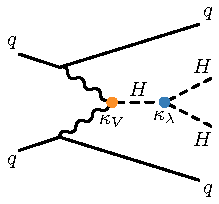
\includegraphics[width=0.48\textwidth]{figures/VBF-diagram-1.pdf}
		 }
\subfloat[]{
		  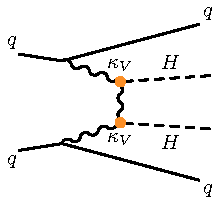
\includegraphics[width=0.48\textwidth]{figures/VBF-diagram-2.pdf}
		 }

\subfloat[]{
		  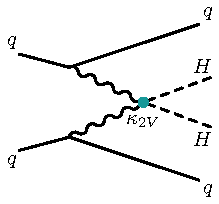
\includegraphics[width=0.48\textwidth]{figures/VBF-diagram-3.pdf}
		 }
\subfloat[]{
		  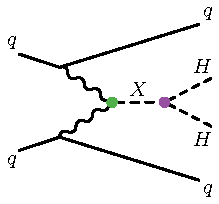
\includegraphics[width=0.48\textwidth]{figures/VBF-diagram-4.pdf}
		 }

\caption{\label{fig:VBF-diagrams} Representative Feynman diagrams for the VBF channel. While this channel may be 
used for both resonant and non-resonant searches~\cite{HDBS-2018-18}, this thesis work was developed concurrently 
with a focused non-resonant search. In addition to variations of the trilinear coupling, $\kappa_{\lambda}$, 
VBF is sensitive to various Higgs couplings to vector bosons, namely $\kappa_{V}$ and $\kappa_{2V}$, attached to 
$VVH$ and $VVHH$ vertices respectively.}
\end{figure} 

The VBF channel proceeds very similarly to the ggF, with the primary differences being the 
kinematic selections and the categorization, which are impacted by the 
presence of two \emph{VBF jets}, resulting from the two initial state quarks. The ggF channel 
result presented here includes a veto on VBF events, such that if events pass the full 
VBF selection, they are not included in the set of events considered for the ggF result.

Beginning with the assumption of four $HH$ jets and two VBF jets, the VBF channel first requires an 
event to have a minimum six jets. The VBF jets are reconstructed as the two jets with the 
highest di-jet invariant mass, $m_{jj}$, out of the set of all non-tagged jets in the event. If no such pair 
exists (i.e., there are less than two non-tagged jets), the event is placed in the ggF channel. 
To reduce the number of background events, three cuts are then applied, VBF jets are required to have 
$\Delta \eta > 3$ and a combined invariant mass of $m_{jj}>$ \SI{1000}{\GeV}. $HH$ jets are identified 
as in the ggF channel, and the vector sum of the $p_{T}$ of the $HH$ and VBF jets is required to be 
less than \SI{65}{\GeV}. The remainder of the analysis proceeds similarly to the ggF channel, and 
events failing any stage of this selection are considered for ggF.

Note that the background estimation for the VBF channel is inherited from the resonant 
and ggF analyses, a significant additional contribution of this thesis work.